%%%%%%%%%%%%%%%%%%%%%%%%%%%%%%%%%%%%%%%%%%%%%%%%%%%%%%%%%%%%%%%%%%%%%%%%
\chapter{Results}
\label{chap:Results}

To show the viability of our tool in the field, we run a small-scale analysis on a small dataset, using a simple research question. We chose this limited approach due to our limited computational budget and time-constraints, but hope to try more in-depth looks in the future. 

For our research question we went with the following: "Are typical conversational threads, in the last three weeks, more negative over all, when looking at online discussions about computer science, in comparison to other topics?". We chose this question, since it follows our intended structure of trying to ask questions about conversational threads in subgroups of a larger conversational space online. Answering this question can be done through our tool as follows:
\begin{enumerate}
    \item Load appropriate data
    \item Filter for data from the last three weeks
    \item Follow typical conversational threads in the larger conversational space
    \item Filter for typical hashtags about computer science, like #computerscience or #CompSci
    \item Compare conversational threads to ones in the larger space
    \item Validate results through look on aggregated statistics
\end{enumerate} 


Finally, we can show unique and interesting findings, which would not have been possible to see without our tool. Figure \ref{fig:example1} shows a typical pattern, which we found often, when looking through the data. The debate, which is held in this thread about the COVID-19 pandemic, keeps a rather negative tone from the bottom up. The conversation however abruptly ends, when a positive connotated message is sent in the end, which can be seen through the bright, green arrow coming down from the top. This pattern of "positive-stops" can be seen in multiple instances and might be an interesting starting point for further research.

\begin{figure}
  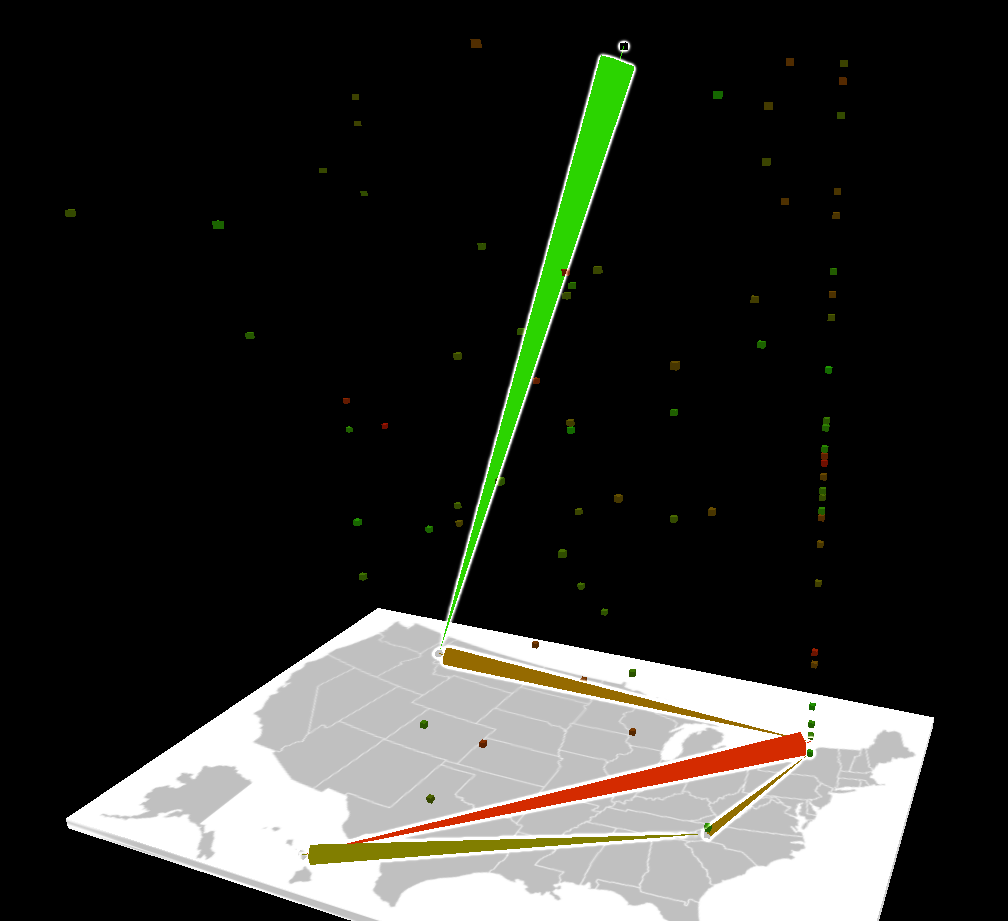
\includegraphics[width=\linewidth]{figures/exempleary.PNG}
  \caption{Rendering with statistics and filters applied. Only cubes are rendered, which do meet the requirements set by the filter. On the left, statistics over the sum of all rendered messages are shown.}
  \label{fig:example1}
\end{figure}
%%%%%%%%%%%%%%%%%%%%%%%%%%%%%%%%%%%%%%%%%%%%%%%%%%%%%%%%%%%%%%%%%%%%%%%%